\subsection{Synthèse des méthodes de compression par extraction de motifs }

	Durant les sections précédentes nous avons expliqué de manière générale les fondements de base de chaque sous-classe de la classe des méthodes de compression par extraction de motifs ainsi que le principe de fonctionnement de leurs méthodes. 
	
	Nous regroupant dans le tableau \ref{enfin} les différentes caractéristiques des méthodes de ces sous-classes. Nous observons qu'elles sont toutes sans perte et destinées aux graphes statiques, à l'exception de la classe des méthodes de compression Basées vocabulaire en utilisant les méthodes de clustering qui contiennent des méthodes de compression supportant les graphes dynamiques. On remarque aussi que la majorité des méthodes de compression par extraction de motifs fournissent en sortie une représentation succincte. Le tableau \ref{enfin} contient aussi un résumé sur les résultats de l'application de ces méthodes que nous représentant dans les figures \ref{comparaison} et \ref{comparaisonVoc}.
	
	La figure \ref{comparaison} illustre les résultats des différentes méthodes de compression basées sur l'agrégation des liens des motifs sous forme de nombre de bits par lien sur le même graphe uk-2002. Elle montre que la sous-classe des méthodes utilisant les techniques de clustering donnent des résultats nettement meilleurs que la sous-classe des méthodes utilisant les règles de grammaire.
	
								\begin{figure}[H]
					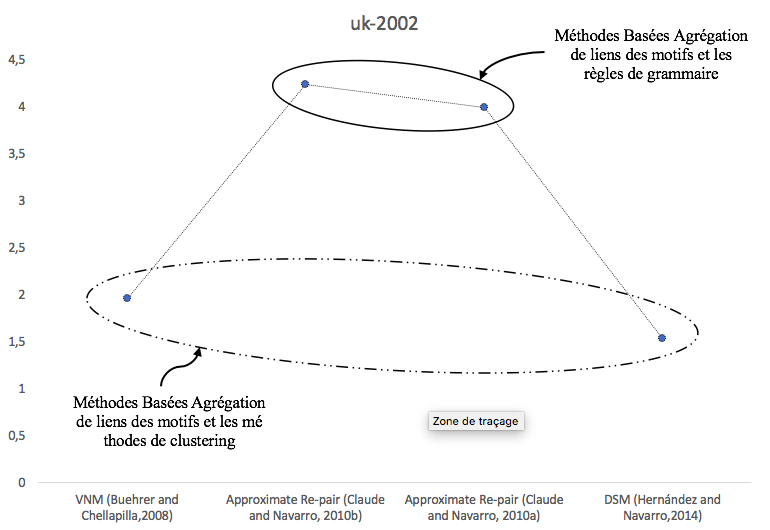
\includegraphics[scale=0.48]{ressources/image/edge.png} 
					\centering
					\caption{Comparaison des performances des méthodes de compression basées sur l'agrégation des liens des motifs}
					\label{comparaison}
				\end{figure}
				
		Tant dis que la figure \ref{comparaisonVoc} 	montre les résultats des taux de compression de la sous-classe des méthodes de compression basées vocabulaire sur deux graphes Enron et uk-2002. Nous remarquons que les résultats sont presque équivalents pour toutes les méthodes et sont autour de 75\%.
				
				\begin{figure}[H]
				
				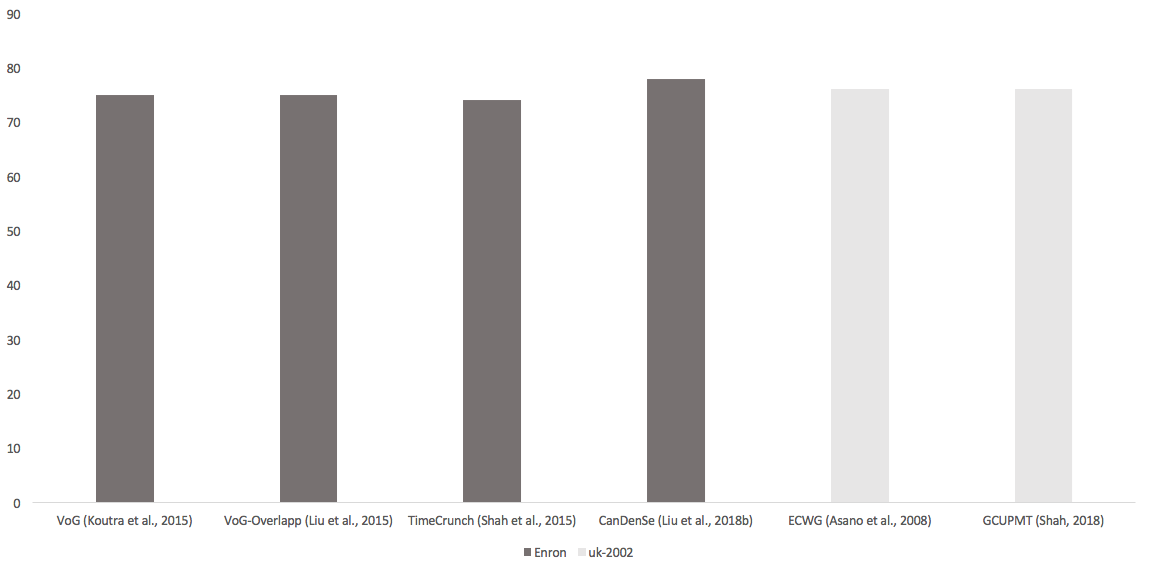
\includegraphics[scale=0.39]{ressources/image/vocabulary.png} 
					\centering
					\caption{Comparaison des performances des méthodes de compression basées vocabulaire}
					\label{comparaisonVoc}
				\end{figure}
			
			

\begin{landscape}
								\begin{table}
								%\renewcommand{\arraystretch}{2}
									\begin{tabular}{|c|C{5.5cm}|c|c|c|c|c|c|c|c|C{2.5cm}|c|}
										\hline
										\multirow{2}{*}[-25pt]{Classe} & \multirow{2}{4cm}[-25pt]{Méthode}  & \multicolumn{4}{c|}{Graphe en entrée} & \multicolumn{2}{c|}{Compression} & \multicolumn{2}{c|}{Structure en sortie}  & \multirow{2}{*}[-25pt]{Graphe de test} & \multirow{2}{*}[-25pt]{Résultat}  \\ \cline{3-10}
				& & \rotatebox[origin=c]{90}{ Orienté }  & \rotatebox[origin=c]{90}{ Non orienté } & \rotatebox[origin=c]{90}{ Statique } & \rotatebox[origin=c]{90}{ Dynamique } & \rotatebox[origin=c]{90}{ Avec perte } & \rotatebox[origin=c]{90}{ Sans perte } & \rotatebox[origin=c]{90}{ Succincte } & \rotatebox[origin=c]{90}{ Structurelle }  & & \\ \hline	 \hline			%%%%%%Fin du header
										
										 \multirow{4}{4cm}{Basée vocabulaire en utilisant  les méthodes de clustering}& VoG \citep{koutra2015summarizing} & \xmark & \cmark & \cmark & \xmark & \xmark & \cmark & \cmark & \xmark  & 
	
	
	Enron									 
			  & 75\%	\\ \cline{2-12}

										 & VoG-Overlapp \citep{liu2015empirical}& \xmark & \cmark & \cmark & \xmark & \xmark &\cmark & \cmark & \xmark  & Enron							 & 75\%	\\  \cline{2-12}
										 & TimeCrunch \citep{shah2015timecrunch}& \xmark & \xmark & \cmark & \cmark & \xmark &\cmark & \cmark & \xmark & 

	
	Enron			&74\%	\\  \cline{2-12}
										 & CanDenSe \citep{liu2018reducing}&     \xmark & \cmark & \xmark & \cmark & \xmark  &\cmark & \cmark & \cmark & Enron									
										 &	 78\%\\ \hline \hline
										 
										 \multirow{2}{4cm}{\footnotesize{Basée vocabulaire en utilisant  les propriétés de la matrice d'adjacence}}&  ECWG
 \citep{asano2008efficient}& \cmark & \cmark & \cmark & \xmark & \xmark &\cmark & \cmark & \xmark  &
	uk-2002	 & 76.1\%	\\  \cline{2-12}
	
	& GCUPMT \citep{shah2018graph} & \cmark & \cmark & \cmark & \xmark & \xmark &\cmark & \cmark & \xmark & 
	graphes 8192 nœuds
							 
			  & 70\%	\\ \hline \hline
			  
			\multirow{2}{4cm}{\small{Basée Agrégation de nœuds des motifs}} & Subdue
 \citep{ketkar2005subdue}& \xmark & \cmark & \cmark & \xmark & \xmark & \cmark & \xmark & \cmark &		
	Graphe des composantes chimiques
										 & 16\%	\\ \cline{2-12}
										 
										 & GraphZip \citep{rossi2018graphzip} & \xmark & \cmark & \cmark & \xmark & \xmark & \cmark & \xmark & \cmark & 
				Web-Google						
								 
			  & 19\%	\\ \hline \hline
			  
			  \multirow{3}{4cm}{Basée Agrégation de liens des motifs en utilisant les règles de grammaire} & Approximate Re-pair
   \citep{claude2010fast}& \cmark & \xmark & \cmark & \xmark & \xmark &  \cmark & \cmark & \xmark	 &		
	uk-2002 & 4.23	\\ \cline{2-12}
	 &  Approximate Re-pair \citep{claude2010extended} & \cmark & \xmark & \cmark & \xmark & \xmark & \cmark & \cmark & \xmark  & 
	uk-2002	 & 3.98 bpe \\	\cline{2-12}
	
	& gRe-pair \citep{maneth2018grammar} & \cmark & \cmark & \cmark & \xmark & \xmark & \cmark & \cmark & \xmark &
  			
  			NotreDame
  			& 4.84 bpe \\ \hline \hline
  			  \multirow{2}{4cm}{\small{Basée Agrégation de liens des motifs et les méthodes de clustering}}& VNM
 \citep{buehrer2008scalable}& \cmark & \xmark & \cmark & \xmark & \xmark & \cmark & \xmark & \cmark &		
	uk-2002 	 & 1.95 bpe \\ \cline{2-12}
	& DSM \citep{hernandez2014compressed} & \cmark & \xmark & \cmark & \xmark &  \xmark & \cmark & \cmark & \cmark  & 
				
	uk-2002 					 
			  & 1.53 bpe	\\
									\hline	 
									\end{tabular}
									\caption{Synthèse des méthodes de compression par extraction de motifs.}
									\label{enfin}									
									
								\end{table}
								
							\end{landscape}
							
							

							
	